\section{Floquet Conductivity in Landau Levels}

Now we can derive conductivity expression for a given Landau level using Floquet conductivity expression derived in [*Ref:my report 2.488]. Before that let's consider the inverse scattering time matrix element in the previous section. From Eq. \eqref{5.3} we can express the $N$th Landau level's inverse scattering time central element ($n=n'=0$) as
\begin{equation} \label{6.1}
  \begin{aligned}
    \qty(\frac{1}{\tau(\varepsilon,k_x)})^{00}_{N} =
    \frac { N_{imp}^2 A^2 \hbar V_{imp}}{16\pi^4 \qty(eB)^2}
    \delta(\varepsilon - \varepsilon_{N}) &
    \int_{-\infty}^{\infty} d {k'}_x \;
    J_0^2\qty(\frac{g\hbar}{eB}[{k}_x - {k'}_x])
    \\
    & \times
    \qty|
    \int_{-\infty}^{\infty} d\bar{k} \;
    {\chi}_{N}\qty(\frac{\hbar}{eB}\bar{k})
    {\chi}_{N}\qty(\frac{\hbar}{eB} \qty[{k'}_x - {k}_x - \bar{k}])|^2.
  \end{aligned}
\end{equation}
Now we can introduce a new parameter with physical meaning of scatterin-induced broading of the Landau level as follows
\begin{equation} \label{6.2}
  \Gamma^{00}_{N}(\varepsilon,k_x) \equiv \hbar \qty(\frac{1}{\tau(\varepsilon,k_x)})^{00}_{N}
\end{equation}
and this modify our previous expressing as
\begin{equation} \label{6.3}
  \begin{aligned}
    \Gamma^{00}_{N}(\varepsilon,k_x)  =
    \frac { N_{imp}^2 A^2 \hbar V_{imp}}{16\pi^4 \qty(eB)^2}
    \delta(\varepsilon - \varepsilon_{N}) &
    \int_{-\infty}^{\infty} d {k'}_x \;
    J_0^2\qty(\frac{g\hbar}{eB}[{k}_x - {k'}_x])
    \\
    & \times
    \qty|
    \int_{-\infty}^{\infty} d\bar{k} \;
    {\chi}_{N}\qty(\frac{\hbar}{eB}\bar{k})
    {\chi}_{N}\qty(\frac{\hbar}{eB} \qty[{k'}_x - {k}_x - \bar{k}])|^2.
  \end{aligned}
\end{equation}
In addition, for the case of elastic scattering within the same Landau level, one can present the delta distribution of the energy using the same physical interpretation as follows
\begin{equation} \label{6.4}
  \delta(\varepsilon - \varepsilon_{N}) \approx
  \frac{1}{\pi \Gamma^{00}_{N}(\varepsilon,k_x)}
\end{equation}
and this leads to
\begin{equation} \label{6.5}
  \begin{aligned}
    \qty[\Gamma^{00}_{N}(\varepsilon,k_x)]^2  =
    \frac { N_{imp}^2 A^2 \hbar V_{imp}}{16\pi^5 \qty(eB)^2}
    \int_{-\infty}^{\infty} d {k'}_x \;
    J_0^2\qty(\frac{g\hbar}{eB}[{k}_x - {k'}_x])
    \qty|
    \int_{-\infty}^{\infty} d\bar{k} \;
    {\chi}_{N}\qty(\frac{\hbar}{eB}\bar{k})
    {\chi}_{N}\qty(\frac{\hbar}{eB} \qty[{k'}_x - {k}_x - \bar{k}])|^2.
  \end{aligned}
\end{equation}
and
\begin{equation} \label{6.6}
  \begin{aligned}
    \Gamma^{00}_{N}(\varepsilon,k_x)  =
    \qty[
    \frac { N_{imp}^2 A^2 \hbar V_{imp}}{16\pi^5 \qty(eB)^2}
    \int_{-\infty}^{\infty} d {k'}_x \;
    J_0^2\qty(\frac{g\hbar}{eB}[{k}_x - {k'}_x])
    \qty|
    \int_{-\infty}^{\infty} d\bar{k} \;
    {\chi}_{N}\qty(\frac{\hbar}{eB}\bar{k})
    {\chi}_{N}\qty(\frac{\hbar}{eB} \qty[{k'}_x - {k}_x - \bar{k}])|^2
    ]^{-1/2}.
  \end{aligned}
\end{equation}
Using the numerical calculations we can see that the above integral is does not depend on the value of $k_x$ and we can choose any values for $k_x$. Therefore applying $k_x =0$ and letting $k'_x \rightarrow k_1,\bar{k}\rightarrow k_2$ we can modify our equation as
\begin{equation} \label{6.7}
  \begin{aligned}
    \Gamma^{00}_{N}(\varepsilon,k_x)  =
    \qty[
    \frac { N_{imp}^2 A^2 \hbar V_{imp}}{16\pi^5 \qty(eB)^2}
    \int_{-\infty}^{\infty} d k_1\;
    J_0^2\qty(\frac{g\hbar}{eB} k_1)
    \qty|
    \int_{-\infty}^{\infty} dk_2 \;
    {\chi}_{N}\qty(\frac{\hbar}{eB} k_2)
    {\chi}_{N}\qty(\frac{\hbar}{eB} \qty[k_1 - k_2])|^2
    ]^{-1/2}.
  \end{aligned}
\end{equation}

\noindent
Now we can compare the central element of energy level broading for each Landau level using normalized Landau energy broading(inverse scattering time) against applied dressing field's electric field's amplitude ($E$) as follows
\begin{equation} \label{6.8}
    \Lambda^{00}_{N} \equiv
    \frac{\Gamma^{00}_{N}(\varepsilon,k_x)}
    {\Gamma^{00}_{N}(\varepsilon,k_x)\big|_{E=0}}.
\end{equation}
As you can see in the Fig. \ref{fig6.1}, when the applied dressing field's intensity is increasing the broading of the Landau energy level decreasing. The effect of this decreasing is depend on the considering Landau level and for higher the level lower the effect.
\begin{figure}[ht!]
  \centering
  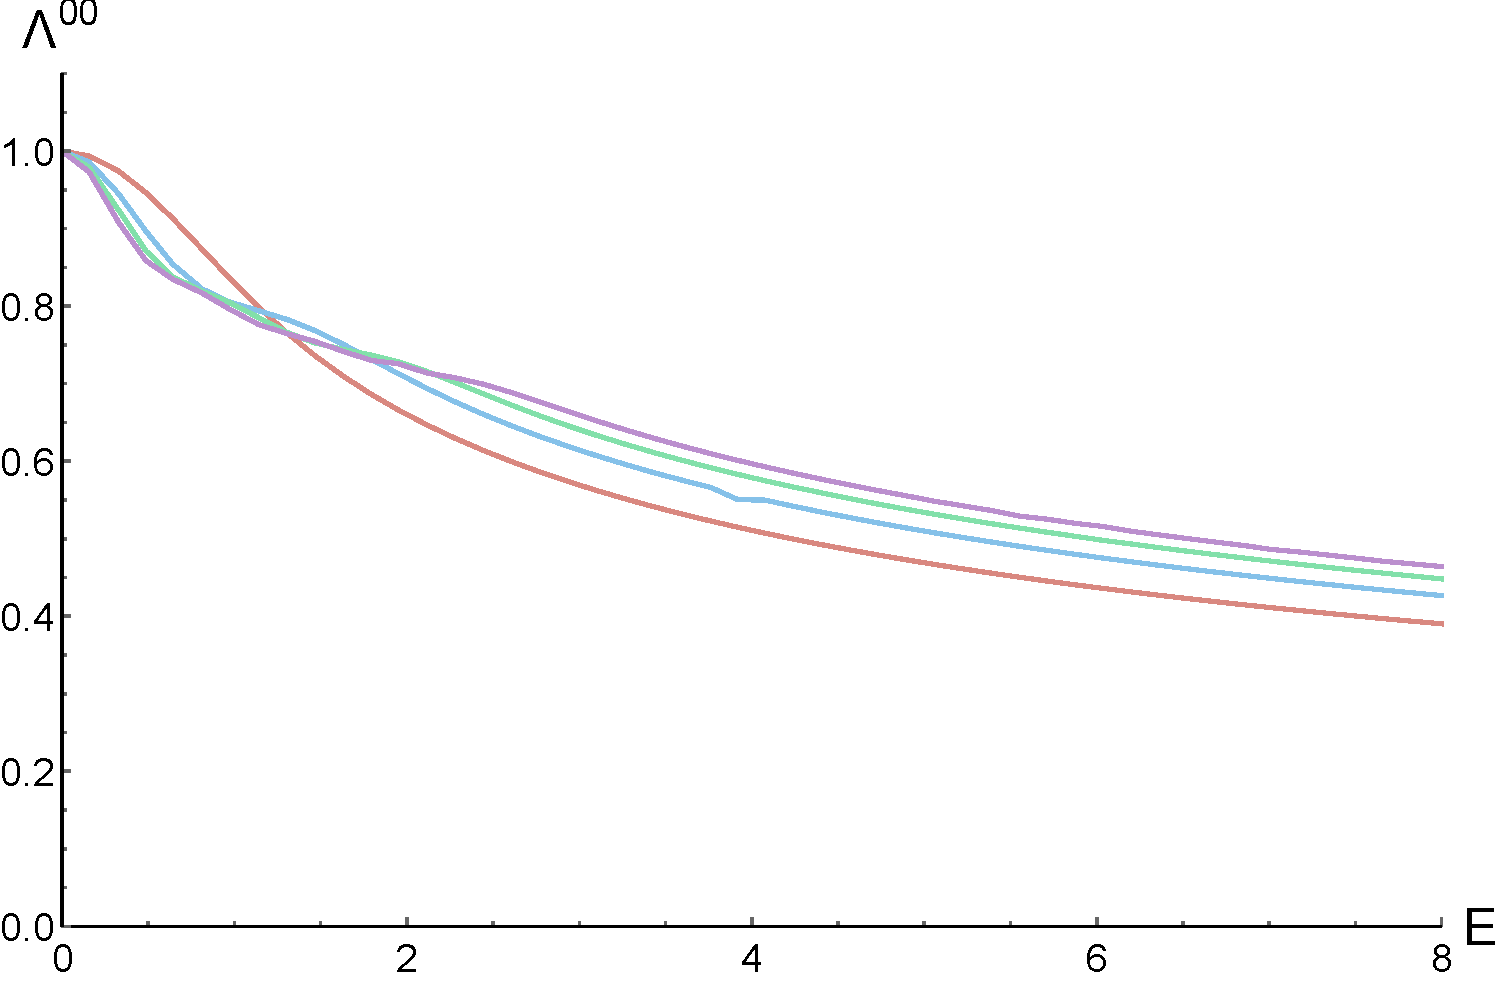
\includegraphics[scale=0.5]{figures/fig04.pdf}
  \caption{Normalized broading of Landau levels agaist dressing fileds amplitude. Red line represents $N=0$, blue line represents $N=1$, green line represents $N=2$ and purplr color line represents $N=3$ Landau levels.}
  \label{fig6.1}
\end{figure}

\noindent
Then we can use Floquet conductivity expression derived in [*Ref:my report 2.488] as follows
\begin{equation} \label{6.9}
  \begin{aligned}
    \lim_{\omega \to 0}
    \text{Re}[{\sigma}^{xx}(0,\omega)] &=
    \frac{-1}{4\pi\hbar A}
    \int_{\lambda-\hbar\Omega/2}^{\lambda+ \hbar\Omega/2} d\varepsilon
    \bigg(
    -\frac{\partial f}{\partial \varepsilon} \bigg)
    \frac{1}{A}\sum_{\mb{k}} \\
    & \times
    \sum_{s,s'=-\infty}^{\infty}
    {j}^x_s(\mb{k}){j}^x_{s'}(\mb{k})
    \tr_s \big[
    \big(
    \mb{G}^{r}_0 (\varepsilon;\mb{k}) - \mb{G}^{a}_0 (\varepsilon;\mb{k})
    \big)
    \odot_s
    \big(
    \mb{G}^{r}_0 (\varepsilon;\mb{k}) - \mb{G}^{a}_0 (\varepsilon;\mb{k})
    \big)
    \big].
  \end{aligned}
\end{equation}
However, in this case we are consider only $x$ directional momentum as a quantum number to seperate different states and let $\lambda = \varepsilon_N$. In addition, with the current operator derivation IF we get component values only for $s=s'=0$ our conductivity rquation will be modified to
\begin{equation} \label{6.10}
  \begin{aligned}
    \lim_{\omega \to 0}
    \text{Re}[{\sigma}^{xx}(0,\omega)] &=
    \frac{-1}{4\pi\hbar A}
    \int_{\varepsilon_N - \hbar\Omega/2}^{\varepsilon_N + \hbar\Omega/2} d\varepsilon
    \bigg(
    -\frac{\partial f}{\partial \varepsilon} \bigg)
    \frac{1}{L_x}\sum_{{k_x}}
    \qty[{j}^x_0({k_x})]^2
    \\
    & \times
    \tr \big[
    \big(
    \mb{G}^{r}_0 (\varepsilon;{k_x}) - \mb{G}^{a}_0 (\varepsilon;{k_x})
    \big)
    \big(
    \mb{G}^{r}_0 (\varepsilon;{k_x}) - \mb{G}^{a}_0 (\varepsilon;{k_x})
    \big)
    \big].
  \end{aligned}
\end{equation}
Now we can expand the above expressing using unitary transformation
\begin{equation} \label{6.11}
    \qty(\mb{T})_{\alpha}^{nn'} \equiv \ket*{\phi_{\alpha}^{n+n'}}
\end{equation}
where
\begin{equation} \label{6.12}
    \ket{\phi_{\alpha}(t)} = \sum_{n = - \infty}^{\infty} e^{-in\omega t}
    \ket{\phi_{\alpha}^{n}}.
\end{equation}
Therefore our conductivity equation becomes
\begin{equation} \label{6.13}
  \begin{aligned}
    \lim_{\omega \to 0}
    \text{Re}[{\sigma}^{xx}(0,\omega)] &=
    \frac{-1}{4\pi\hbar A}
    \int_{\varepsilon_N - \hbar\Omega/2}^{\varepsilon_N + \hbar\Omega/2} d\varepsilon
    \bigg(
    -\frac{\partial f}{\partial \varepsilon} \bigg)
    \frac{1}{L_x}\sum_{{k_x}}
    \qty[{j}^x_0({k_x})]^2
    \\
    & \times
    \qty[
    \mb{T}^{\dagger}(k_x)
    \big(
    \mb{G}^{r}_0 (\varepsilon;{k_x}) - \mb{G}^{a}_0 (\varepsilon;{k_x})
    \big)
    \mb{T})(k_x)
    ]^2_{00}.
  \end{aligned}
\end{equation}
As derived in [*Ref:my report 2.547] we can present this matrix multiplication result as follows
\begin{equation} \label{6.14}
  \begin{aligned}
    \qty[
    \mb{T}^{\dagger}(k_x)
    \big(
    \mb{G}^{r}_0 (\varepsilon;{k_x}) - \mb{G}^{a}_0 (\varepsilon;{k_x})
    \big)
    \mb{T})(k_x)
    ]^2_{00} &
    \approx
    \qty[
    \mb{T}^{\dagger}(k_x)
    \big(
    \mb{G}^{r}_0 (\varepsilon;{k_x})\mb{G}^{a}_0 (\varepsilon;{k_x})
    \big)
    \mb{T})(k_x)
    ]_{00} \\
    & =
    \frac{-1}
    {
      \qty(\frac{\varepsilon}{\hbar} - \frac{\varepsilon_N}{\hbar})^2
      +
      \qty(\frac{\Gamma^{00}_{N}(\varepsilon,k_x)}{2\hbar})^2
    }
  \end{aligned}
\end{equation}
and this can be more simplified as
\begin{equation} \label{6.15}
  \begin{aligned}
    \qty[
    \mb{T}^{\dagger}(k_x)
    \big(
    \mb{G}^{r}_0 (\varepsilon;{k_x}) - \mb{G}^{a}_0 (\varepsilon;{k_x})
    \big)
    \mb{T})(k_x)
    ]^2_{00} =
    \frac{-\hbar^2}
    {\qty[\Gamma^{00}_{N}(\varepsilon,k_x)]^2}
    \qty[
      1 +
      \qty(\frac{{\varepsilon}-{\varepsilon_N}}{\Gamma^{00}_{N}(\varepsilon,k_x)/2})^2
    ]^{-1}.
  \end{aligned}
\end{equation}
Since the squared termed in the square brackets goinf to zero with valid conditions we can use binomial approximation for the square bracket term and get the following derivation
\begin{equation} \label{6.16}
  \begin{aligned}
    \qty[
    \mb{T}^{\dagger}(k_x)
    \big(
    \mb{G}^{r}_0 (\varepsilon;{k_x}) - \mb{G}^{a}_0 (\varepsilon;{k_x})
    \big)
    \mb{T})(k_x)
    ]^2_{00} =
    \frac{-\hbar^2}
    {\qty[\Gamma^{00}_{N}(\varepsilon,k_x)]^2}
    \qty[
      1 -
      4\qty(\frac{{\varepsilon}-{\varepsilon_N}}{\Gamma^{00}_{N}(\varepsilon,k_x)})^2
    ]
  \end{aligned}
\end{equation}

\noindent
Now the conductivity expression get modify as
\begin{equation} \label{6.17}
  \begin{aligned}
    \lim_{\omega \to 0}
    \text{Re}[{\sigma}^{xx}(0,\omega)] =
    \frac{\hbar}{4\pi A L_x}
    \int_{\varepsilon_N - \hbar\Omega/2}^{\varepsilon_N + \hbar\Omega/2} d\varepsilon
    \bigg(
    -\frac{\partial f}{\partial \varepsilon} \bigg)
    \sum_{{k_x}}
    \qty[{j}^x_0({k_x})]^2
    \frac{\hbar^2}
    {\qty[\Gamma^{00}_{N}(\varepsilon,k_x)]^2}
    \qty[
      1 -
      4\qty(\frac{{\varepsilon}-{\varepsilon_N}}{\Gamma^{00}_{N}(\varepsilon,k_x)})^2
    ]
  \end{aligned}
\end{equation}

\noindent
Then assuming we are considering fermions in aero temperature for this scenario we can describe the particle distribution function using the Fermi-Dirac distribution in zero-tempurature.
\begin{equation} \label{6.18}
    -\frac{\partial f}{\partial \varepsilon} = \delta(\varepsilon_F - \varepsilon)
\end{equation}
where $\varepsilon_F$ represent the Fermi energy for the considered material.

\noindent
With this approximation we can derive that
\begin{equation} \label{6.19}
  \begin{aligned}
    \lim_{\omega \to 0}
    \text{Re}[{\sigma}^{xx}(0,\omega)] =
    \frac{\hbar}{4\pi A L_x}
    \int_{\varepsilon_N - \hbar\Omega/2}^{\varepsilon_N + \hbar\Omega/2} d\varepsilon
    \delta(\varepsilon_F - \varepsilon)
    \sum_{{k_x}}
    \qty[{j}^x_0({k_x})]^2
    \frac{\hbar^2}
    {\qty[\Gamma^{00}_{N}(\varepsilon,k_x)]^2}
    \qty[
      1 -
      4\qty(\frac{{\varepsilon}-{\varepsilon_N}}{\Gamma^{00}_{N}(\varepsilon,k_x)})^2
    ]
  \end{aligned}
\end{equation}
and
\begin{equation} \label{6.20}
  \begin{aligned}
    \lim_{\omega \to 0}
    \text{Re}[{\sigma}^{xx}(0,\omega)] =
    \frac{\hbar}{4\pi A L_x}
    \sum_{{k_x}}
    \qty[{j}^x_0({k_x})]^2
    \frac{\hbar^2}
    {\qty[\Gamma^{00}_{N}(\varepsilon_F,k_x)]^2}
    \qty[
      1 -
      4\qty(\frac{{\varepsilon_F}-{\varepsilon_N}}{\Gamma^{00}_{N}(\varepsilon_F,k_x)})^2
    ]
  \end{aligned}
\end{equation}


























\hfill$\blacksquare$
